% =========================================================================== %
% Eclipse Basics
% =========================================================================== %

\ifx\wholebook\relax\else
  \documentclass[a4paper,10pt,twoside]{book}
  %=============================================================================%
% Common things, settings, packages to include
%=============================================================================%

\usepackage{graphicx}
\usepackage{color}
\usepackage{makeidx}
\usepackage{ifpdf}
\usepackage{verbatim}

% --------------------------------------------------------------------------- %
% Setting up stuff depeding on output format
% --------------------------------------------------------------------------- %

\ifpdf
  % special settings for pdf mode
  \usepackage[colorlinks]{hyperref}
  \usepackage{courier}
  
  \hypersetup{
    colorlinks,
    linkcolor=darkblue,
    citecolor=darkblue,
    pdftitle={The Eclipse Scout Book},
    pdfauthor={The Scout Community},
    pdfkeywords={Enterprise Framework, Eclipse, Java, Client-Side, Rich Client, Web Client, Mobile},
    pdfsubject={Computer Science}
  }
  
  \usepackage{caption}
  \captionsetup{margin=10pt,font=small,labelfont=bf}
\else
  % special stuff for html mode
  \usepackage[tex4ht]{hyperref}
\fi

% --------------------------------------------------------------------------- %
% Setting up printing range
% --------------------------------------------------------------------------- %

\parindent 1cm
\parskip 0.2cm
\topmargin 0.2cm
\oddsidemargin 1cm
\evensidemargin 0.5cm
\textwidth 15cm
\textheight 21cm

% --------------------------------------------------------------------------- %
% Setting up listings
% --------------------------------------------------------------------------- %

\usepackage{listings}
 
\definecolor{darkviolet}{rgb}{0.5,0,0.4}
\definecolor{darkgreen}{rgb}{0,0.4,0.2} 
\definecolor{darkblue}{rgb}{0.1,0.1,0.9}
\definecolor{darkgrey}{rgb}{0.5,0.5,0.5}
\definecolor{lightblue}{rgb}{0.4,0.4,1}
\definecolor{lightgray}{rgb}{0.97,0.97,0.97}

\renewcommand{\lstlistlistingname}{List of Listings}

% general settings
\lstset{
  basicstyle=\small\ttfamily,
  columns=fullflexible,
  breaklines=true,
  breakindent=10pt,
  prebreak=\mbox{{\color{blue}\tiny$\searrow$}},
  postbreak=\mbox{{\color{blue}\tiny$\rightarrow$}},
  showstringspaces=false,
  backgroundcolor=\color{lightgray}
}

% settings for xml files
\lstdefinelanguage{xml}
{
  commentstyle=\color{darkgrey}\upshape,
  morestring=[b]",
  morestring=[s]{>}{<},
  morecomment=[s]{<?}{?>},
  stringstyle=\color{black},
  identifierstyle=\color{darkblue},
  keywordstyle=\color{cyan},
  morekeywords={xmlns,name,point,factory,class}% list your attributes here
}

% settings for ini files
\lstdefinelanguage{ini}
{
  morecomment=[f][\color{darkgrey}\upshape][0]\#, % # is comment iff it's the first char on the line
  stringstyle=\color{black}
}

% default settings (for java files)
\lstset{
  language=Java,
  emphstyle=\color{red}\bfseries,
  keywordstyle=\color{darkviolet}\bfseries,
  commentstyle=\color{darkgreen},
  morecomment=[s][\color{lightblue}]{/**}{*/},
  stringstyle=\color{darkblue},
}

% --------------------------------------------------------------------------- %
% cross reference macros
% --------------------------------------------------------------------------- %
\newcommand{\applabel}[1]{\label{apx:#1}}
\newcommand{\chalabel}[1]{\label{cha:#1}}
\newcommand{\seclabel}[1]{\label{sec:#1}}
\newcommand{\lstlabel}[1]{\label{lst:#1}}
\newcommand{\figlabel}[1]{\label{fig:#1}}
\newcommand{\tablabel}[1]{\label{tab:#1}}

\newcommand{\appref}[1]{Appendix~\ref{apx:#1}}
\newcommand{\charef}[1]{Chapter~\ref{cha:#1}\xspace}
\newcommand{\secref}[1]{Section~\ref{sec:#1}}
\newcommand{\lstref}[1]{Listing~\ref{lst:#1}\xspace}
\newcommand{\figref}[1]{Figure~\ref{fig:#1}\xspace}
\newcommand{\tabref}[1]{Table~\ref{tab:#1}\xspace}

% --------------------------------------------------------------------------- %
% graphics paths
% --------------------------------------------------------------------------- %
\graphicspath{
  {figures/}
  {Introduction/figures/}
}

%=============================================================================%

  \pagestyle{headings}
  \graphicspath{{figures/} {../figures/}}
  \begin{document}
  \sloppy
\fi


% --------------------------------------------------------------------------- %
\chapter{Eclipse Basics}
\applabel{eclipse_basics}

% --------------------------------------------------------------------------- %
\section{Eclipse as an IDE}
\applabel{eclipse_ide}

Excellent Eclipse IDE tutorial by L. Vogel \url{http://www.vogella.com/articles/Eclipse/article.html}.

\subsection{Project Workspace}

% ........................................................................... %
\subsection{Perspectives}
\applabel{eclipse_perspective}

A perspective contains the visual elements and the arrangement of those elements to support a specific development task within the Eclipse IDE. 
Perspectives relevant to the development of Scout applications are the Scout perspective, the Java perspective, the Debug perspective, and many others. 
To open a perspective available in the Eclipse IDE, the \button{Open Perspective} or the \menu{Window $\rightarrow$ Open Perspective $\rightarrow$ Other...} can be used. 

\begin{figure}
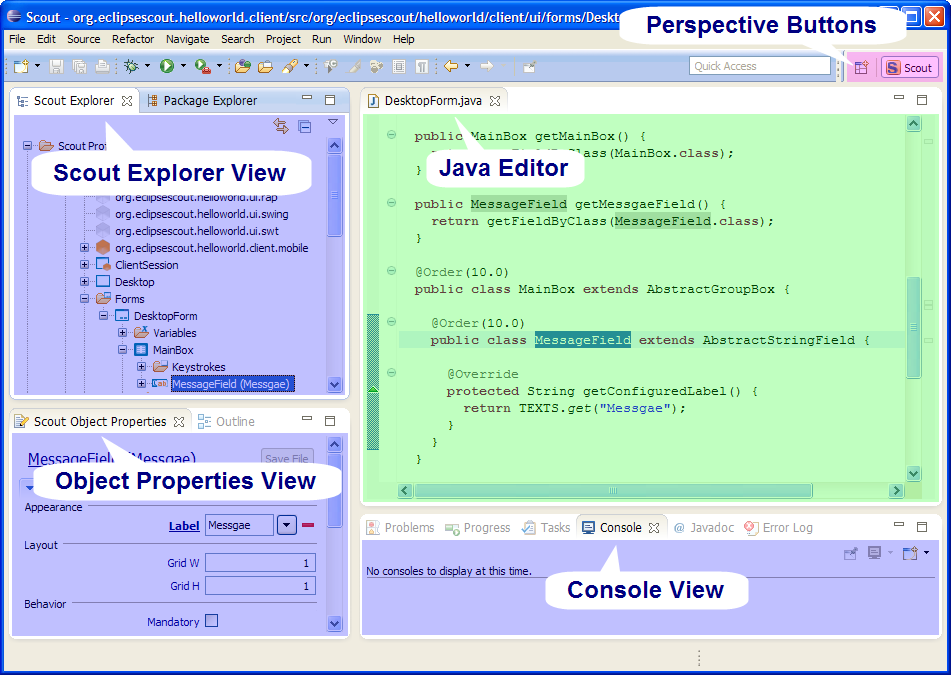
\includegraphics[width=14cm]{eclipse_ide_parts.png} 
\caption{The Eclipse IDE with the Scout perspective. The colors indicate the different elements. View parts (blue), editor parts (green) and perspective buttons (purple). }
\figlabel{eclipse_ide_parts}
\end{figure}

\figref{eclipse_ide_parts} provides a screenshot of the Eclipse Scout perspective indicating the corresponding perspective button and the main view parts and editor parts involved. 
Using drag and drop, views and editors can be freely moved around in the Eclipse IDE to suit the developer's needs.
Perspectives can be further individualized using the \menu{Window $\rightarrow$ Customize Perspective...}. 
Here, the visibility of the toolbar items and menu entries can be defined. 
Once a suitable layout of all desired elements has been defined, this organisation may be saved as a personal perspective using the Eclipse IDE \menu{Window $\rightarrow$ Save Perspective As...}.

In case a customizing step does not turn out as intended, with the \menu{Window $\rightarrow$ Reset Perspective...} is always possible to go back to the last saved state of the current perspective.

% --------------------------------------------------------------------------- %
\section{OSGi and Equinox}
\applabel{osgi_basics}

\fbox{
  \parbox{12cm}{
    Section waiting for contribution (2'000-3'000 words).
 
    The goal of this section is to provide the reader with a solid overview of OSGi concepts and its Equinox implementation. 
    Where appropriate, provide links to high quality online material, that is likely to exist for at least the next year or two.
  }
}

What is OSGi: \url{http://www.osgi.org/Technology/WhatIsOSGi}
What is Equinox: \url{http://www.eclipse.org/equinox/}



Server-side Equinox: \url{http://www.eclipse.org/equinox/server/http_in_container.php}

The web.xml, the lib/servletbridge.jar and eclipse/plugins/servlet, equinox and bla stuff

bundle example


needs text

  * bundles
  * services
  * classloading
  
% --------------------------------------------------------------------------- %
\section{Eclipse}
\applabel{platform_basics}

\fbox{
  \parbox{12cm}{
    Section waiting for contribution (3'000-6'000 words).
    
    The goal of section is to provide the reader with a solid overview of standard Eclipse concepts relevant for scout projects and central parts of the Scout framework and Scout SDK tooling. 
    where appropriate, provide links to high quality online material that is likely to exist for at least the next year or two
  }
}

needs text

% ........................................................................... %
\section{Eclipse Plugins}
\applabel{plugin_basics}

release engineering artefacts vs runtime artefacts. start with runtime artefacts

  * plugins
  * fragments
  * features
  * products
  * targets
  * servlet bridge
  * client exe files
  
% --------------------------------------------------------------------------- %
  
\ifx\wholebook\relax\else
   \begin{thebibliography}{99}
  \addcontentsline{toc}{chapter}{Bibliography}
  
  % add/insert books in alphabetical order of 1st author
  
  \bibitem{batessierra05}
    \textit{Bert Bates, Kathy Sierra},
	\textbf{Head First Java} 2nd edition, 
	O'Reilly Media, 2005.

  \bibitem{bloch08} 
    \textit{Joshua Bloch},
    \textbf{Effective Java} 2nd edition, 
	Addison-Wesley, 2008.
	
  \bibitem{eckel06}
    \textit{Bruce Eckel},
	\textbf{Thinking in Java} 4th edition, 
	Prentice Hall International, 2006.

\end{thebibliography}

   \end{document}
\fi

% =========================================================================== %
